\section{Технологическая часть}
В данной части рассматривается выбор средств реализации, описывается структура классов программы и приводится интерфейс программного обеспечения.

\subsection{Средства реализации}

Для написания данной курсовой работы был выбран язык C++~\cite{cpp-lang}.
Выбор данного языка программирования обусловлен следующим образом:
\begin{itemize}
	\item C++ --- объектно-ориентированный язык, а именно такая методология
	программирования была выбрана для разработки программы;
	\item в данном языке имеется большое количество библиотек и шаблонов,
	позволяющих не тратить время на изобретение готовых конструкций.;
	\item обладает высокими показателями вычислительной производительности, а так как требуется быстродействие задач генерации реалистичных изображений, то язык C++ необходим.
\end{itemize}

В качестве среды разработки был использован Qt Creator~\cite{qt-creator}.
Данный выбор обусловлен следующими факторами:
\begin{itemize}
	\item в QT Creator есть возможность быстрого создания интерфейса с помощью расширения QT Design;
	\item QT Creator обладает всем необходимым функционалом для написания, профилирования и отладки программ.
\end{itemize}

\subsection{Описание структуры программы}

На рисунке~\ref{fig:struct} представлена схема разработанных классов.

\begin{figure}[h]
	\centering
	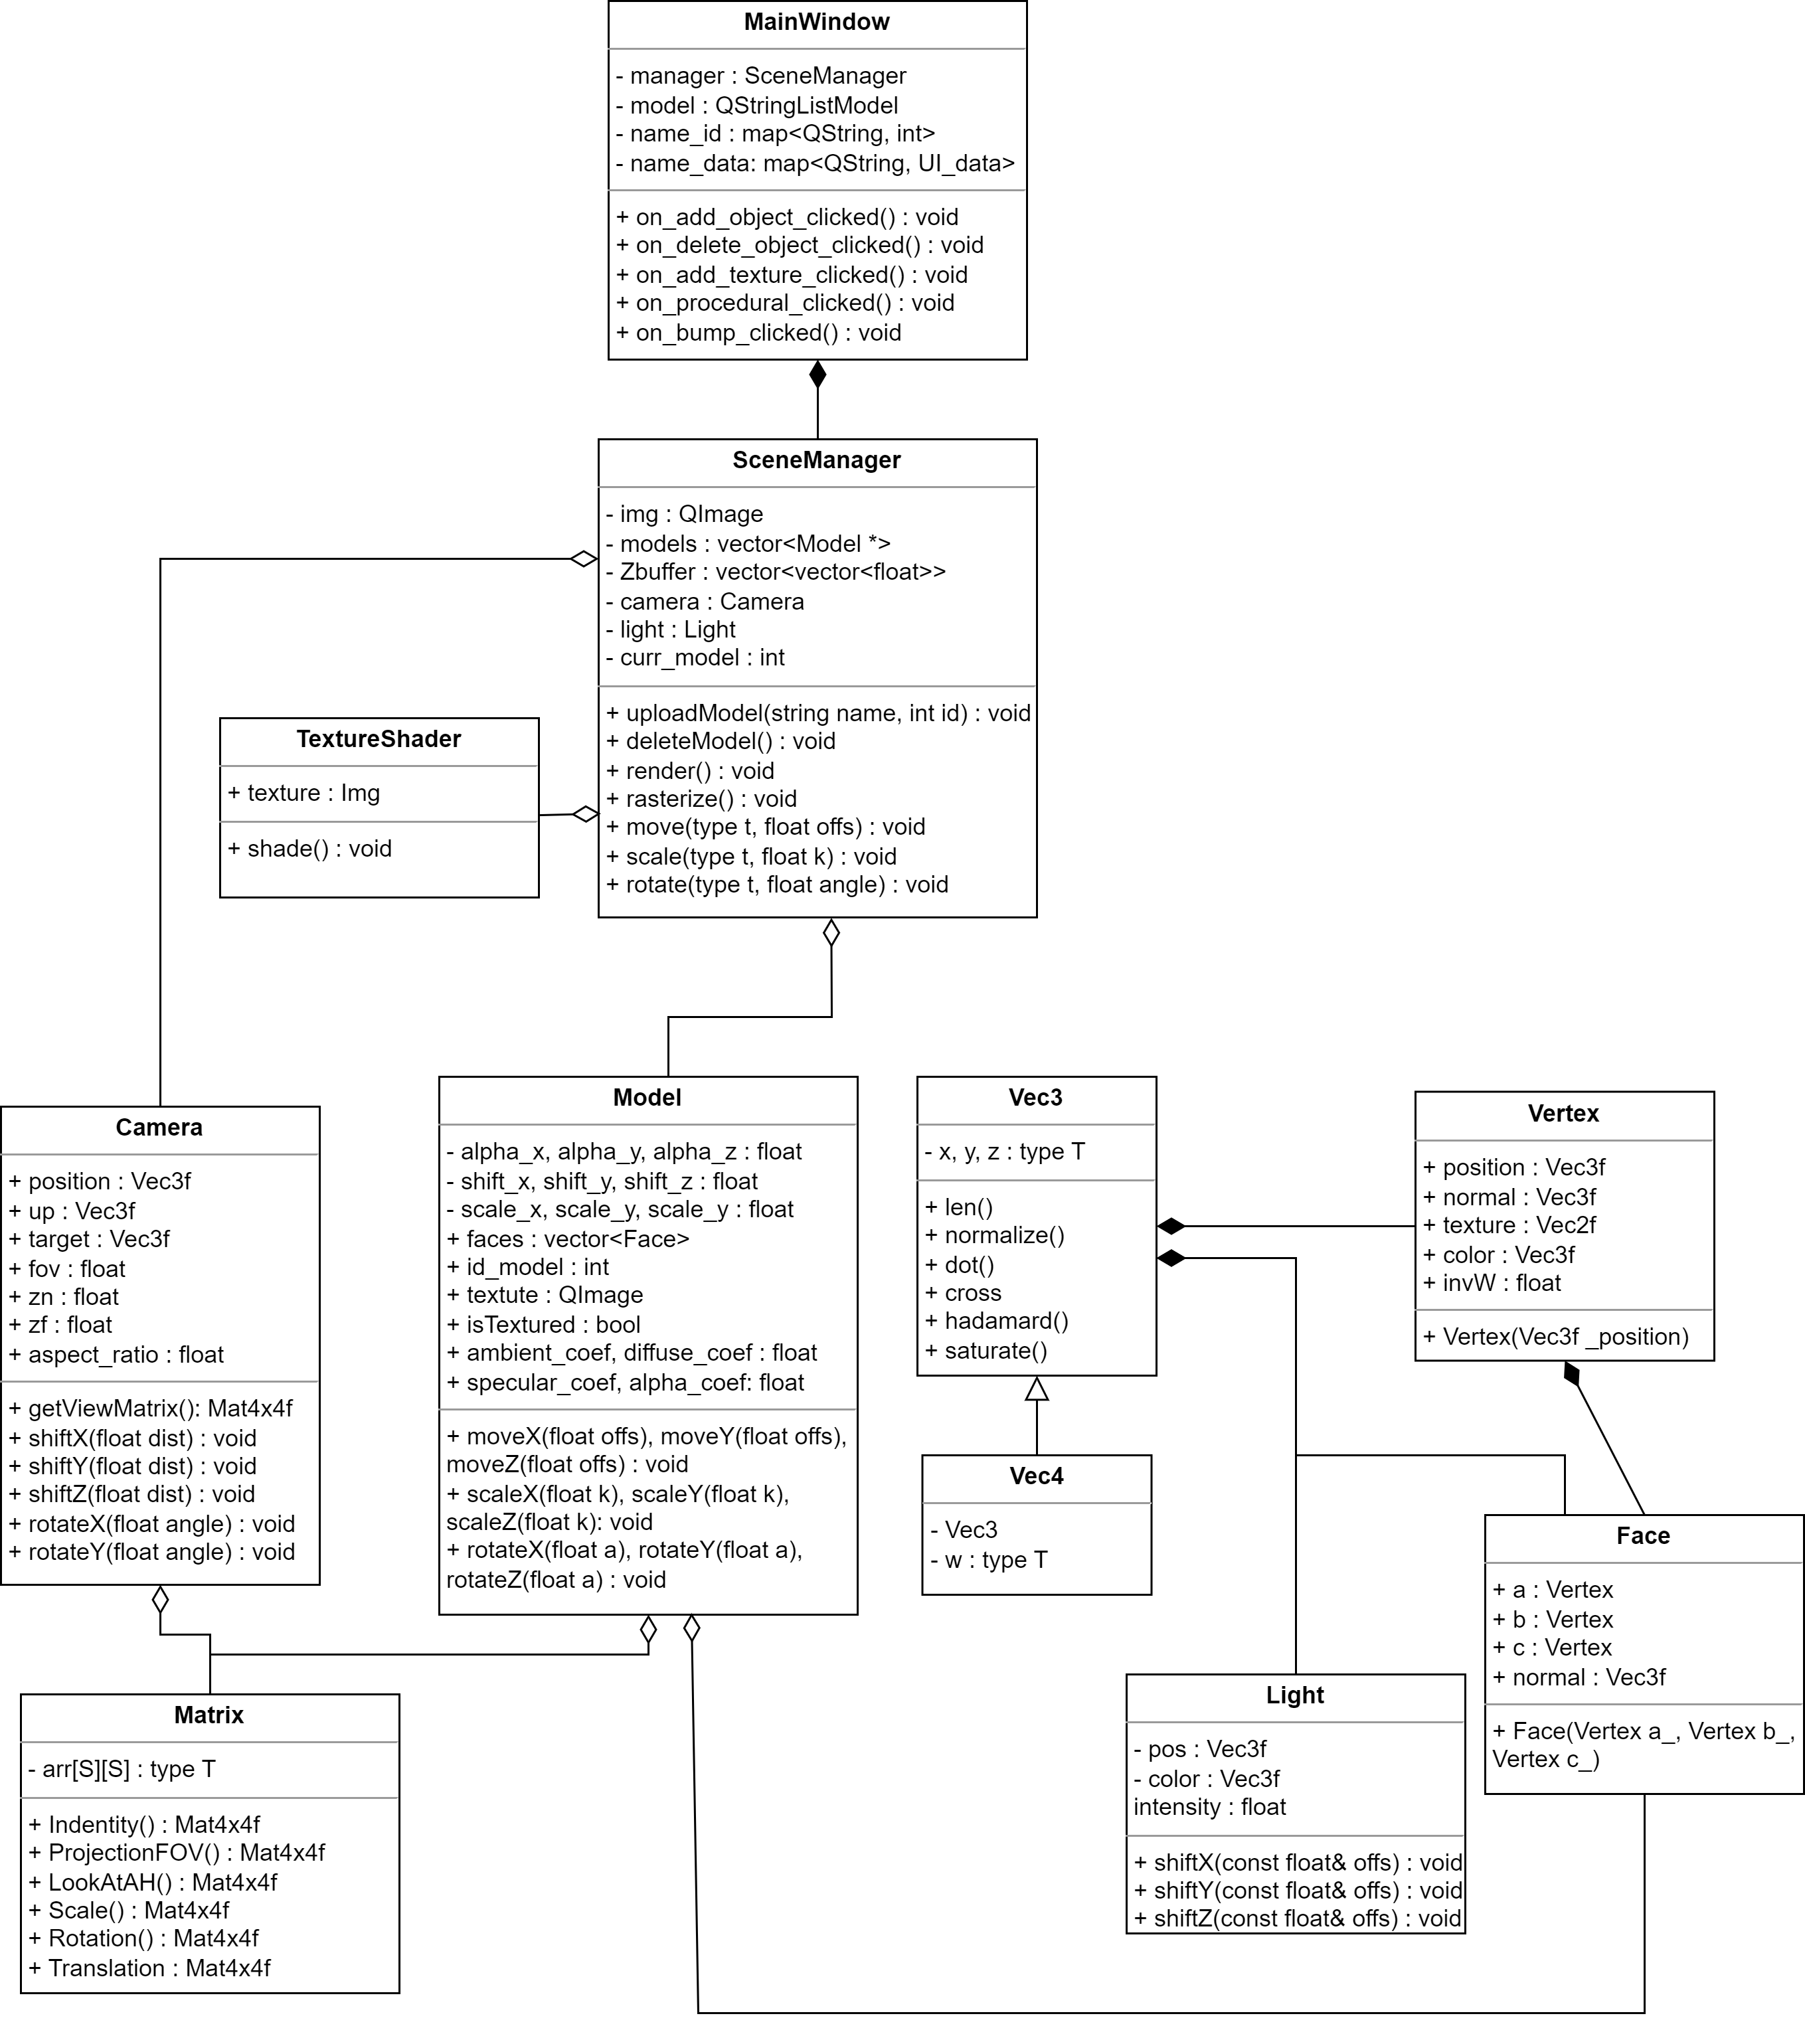
\includegraphics[width=0.9\textwidth]{img/algorithms/struct.png}
	\caption{Схема классов программы}
	\label{fig:struct}
\end{figure}
\clearpage
В программе реализованы следующие классы:
\begin{itemize}
	\item class SceneManager --- хранит сцену, описывает методы взаимодействия со сценой и объектами на ней;
	\item class Model --- описывает представление трёхмерного объекта и методы работы с ним;
	\item class Light --- описывает источники света и методы взаимодействия с ним;
	\item class Camera --- описывает камеру и методы взаимодействия с ней;
	\item class Vector --- реализация векторов размерности 3 и 4;
	\item class Matrix --- описывает матрицы и методы взаимодействия с ними.
	\item class TextureShader --- содержит функции для интерполяции значения текстурных координат в конкретном пикселе;
\end{itemize}

\subsection{Реализация алгоритмов}
\begin{lstinputlisting}[
	caption={Алгоритм растеризации каждого объекта},
	label={lst:rasterize_object},
	linerange={71-86}
	]{../src/scene_manager.cpp}
\end{lstinputlisting}

\begin{lstinputlisting}[
	caption={Алгоритм растеризации треугольника},
	label={lst:rasterize_triangle},
	linerange={33-69}
	]{../src/scene_manager.cpp}
\end{lstinputlisting}

\begin{lstinputlisting}[
	caption={Алгоритм преобразования вершин в экранное пространство},
	label={lst:conver_vertex},
	linerange={5-28}
	]{../src/shader.cpp}
\end{lstinputlisting}

\begin{lstinputlisting}[
	caption={Алгоритм текстуризации},
	label={lst:texture},
	linerange={10-35}
	]{../src/texture.cpp}
\end{lstinputlisting}

\subsection{Описание интерфейса программного обеспечения}
На рисунке \ref{fig:interface} представлен стартовый экран программы.
Он предоставляет пользователю возможность добавить объект, изменить положение источника света и ёго интенсивность.
\begin{figure}[h]
	\centering
	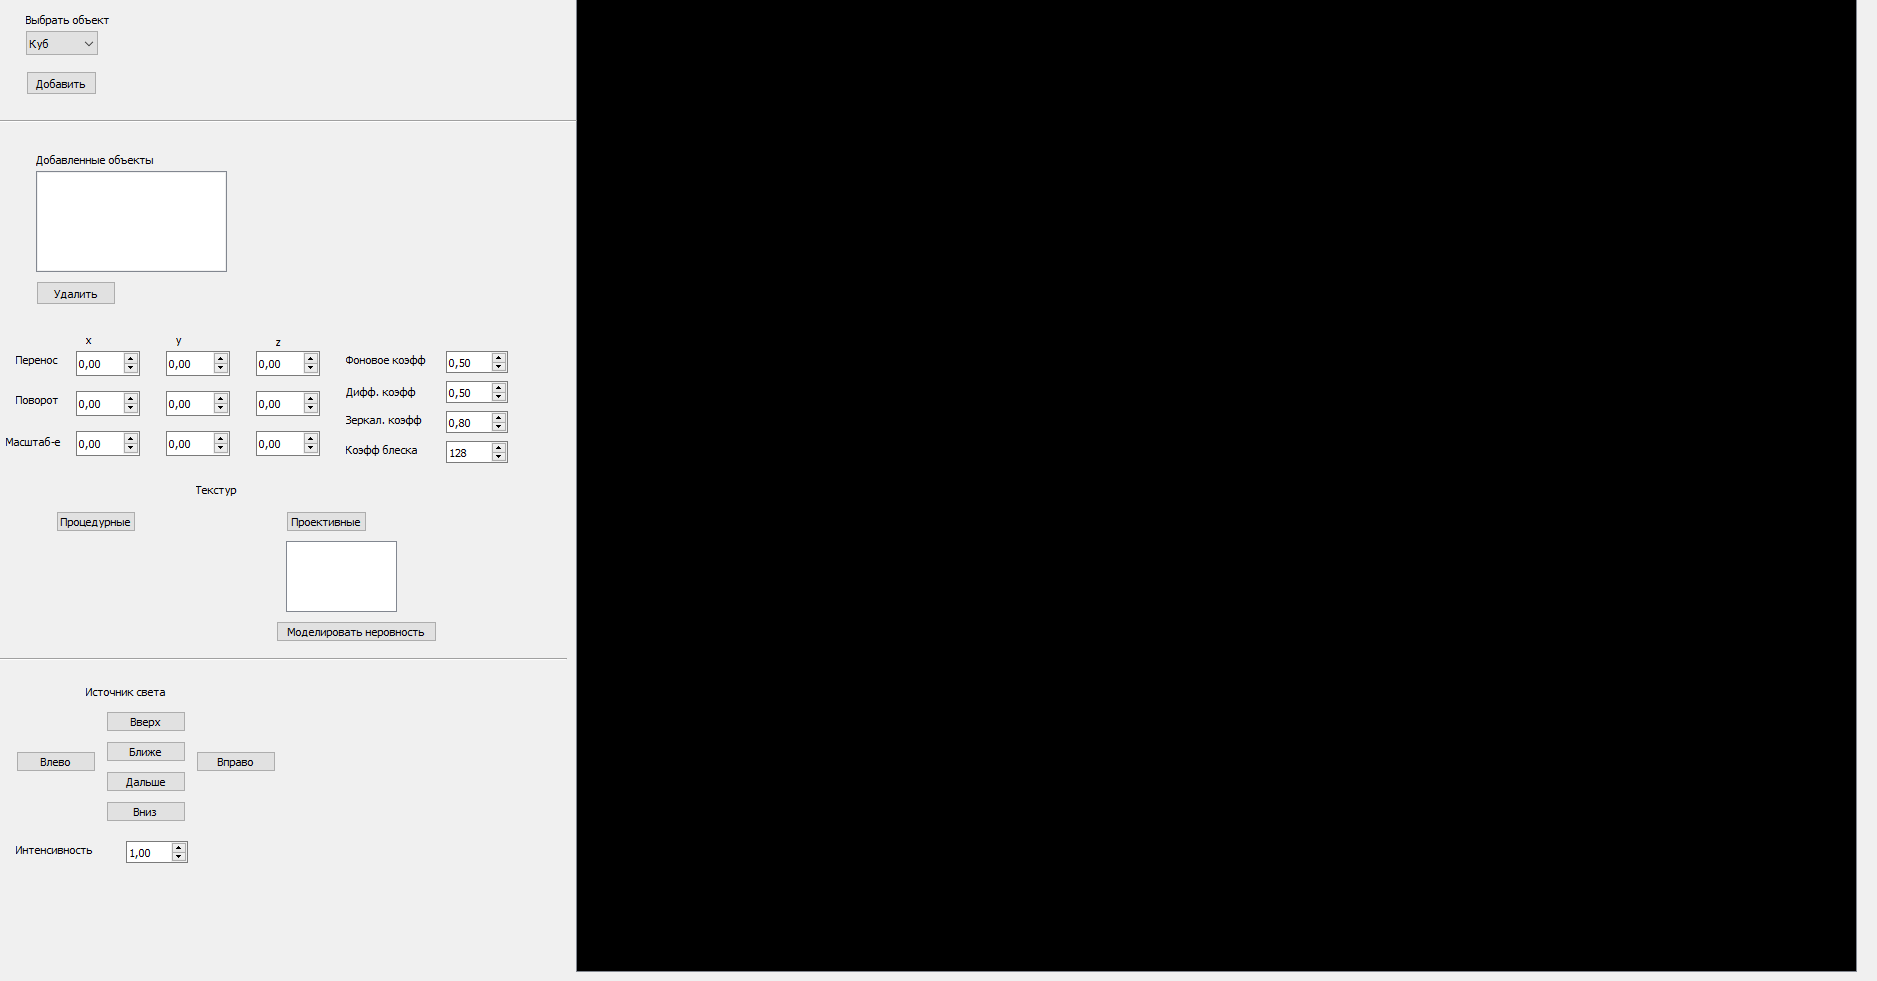
\includegraphics[width=0.95\textwidth]{img/examples/interface.png}
	\caption{Пользовательский интерфейс}
	\label{fig:interface}
\end{figure}

Для добавления объекта модели её нужно выбрать в выпадающем меню в левом верхнем углу, а затем нажать на кнопку добавления. Модель появится на графике, а также в текстовом поле.
Для наложения текстур на объект, нужно выбрать объект из списки, а затем нажать либо на кнопку <<Процедурные>> либо на кнопку <<Проективные>>.
Для моделирования неровностей нажать на кнопку <<Моделировать неровности>>.
Управление камерой осуществляется при помощи клавиатуры кнопками W, A, S, D, H, K, U, J.

\subsection{Демонстрация работы программы}
На рисунках \ref{fig:demon1}--\ref{fig:demon3} представлены результаты работы программы.
\clearpage
\begin{figure}[h]
	\centering
	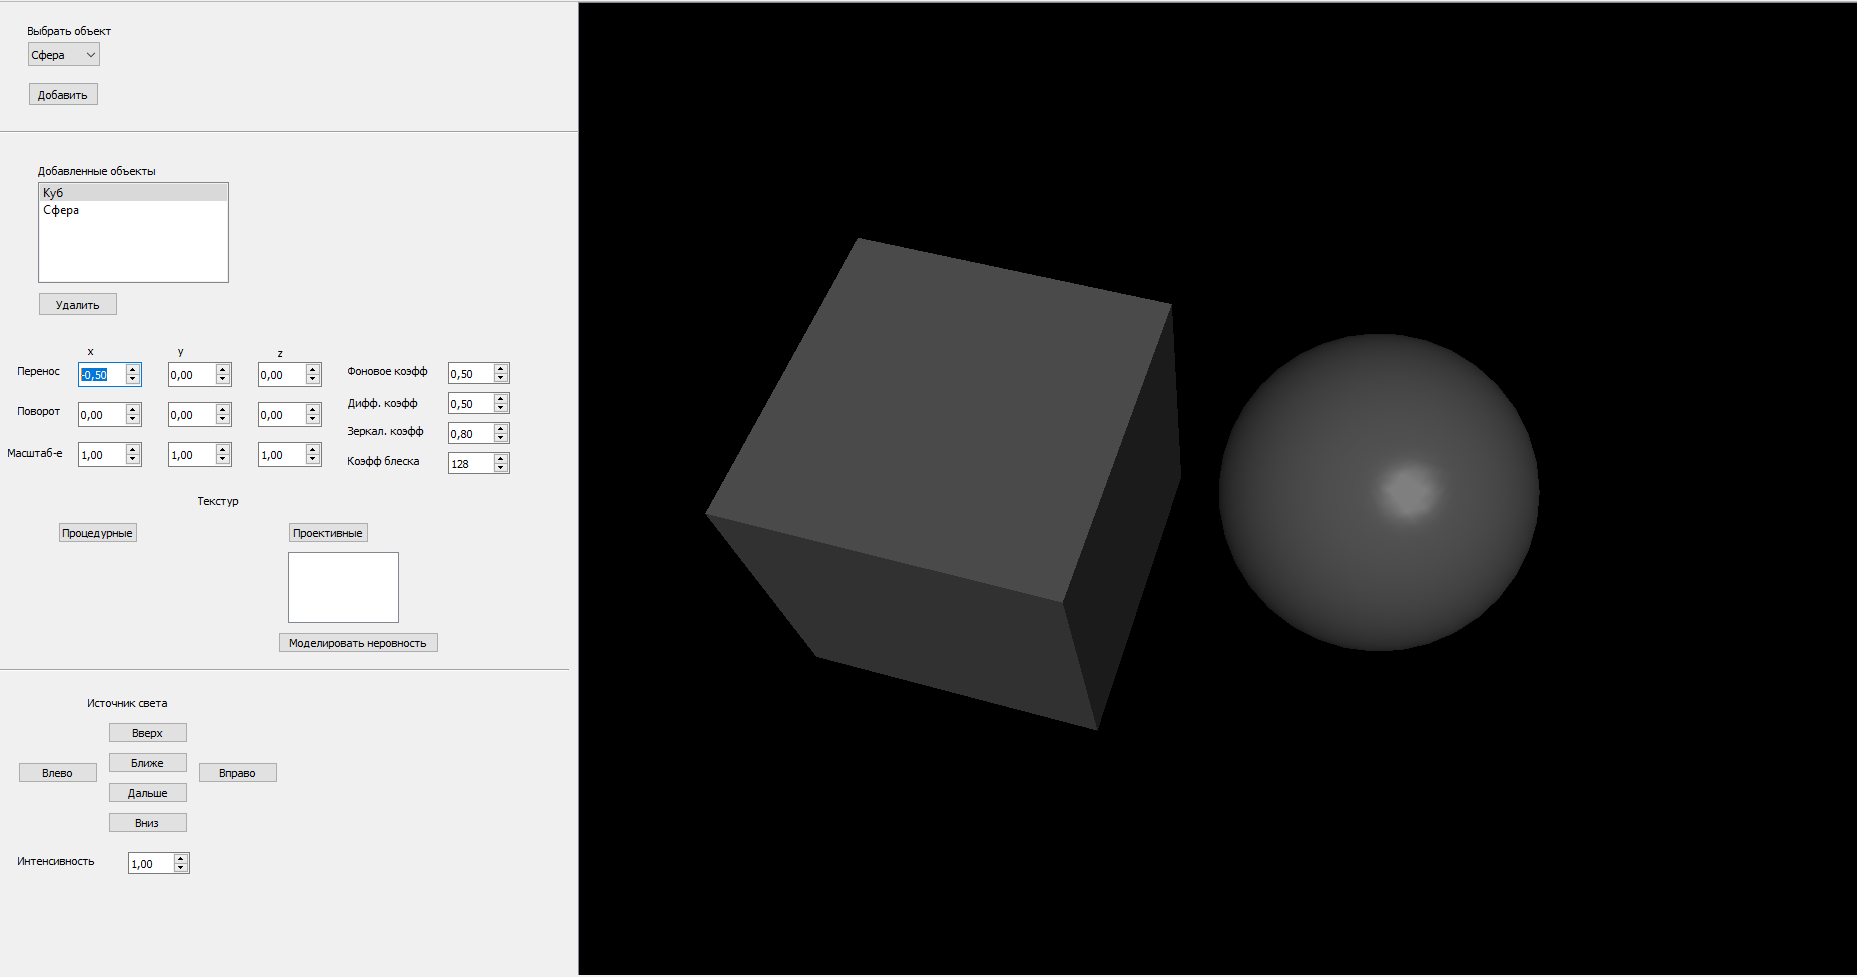
\includegraphics[width=0.95\textwidth]{img/examples/demon1.png}
	\caption{Результат работы программы без текстуры}
	\label{fig:demon1}
\end{figure}

\begin{figure}[h]
	\centering
	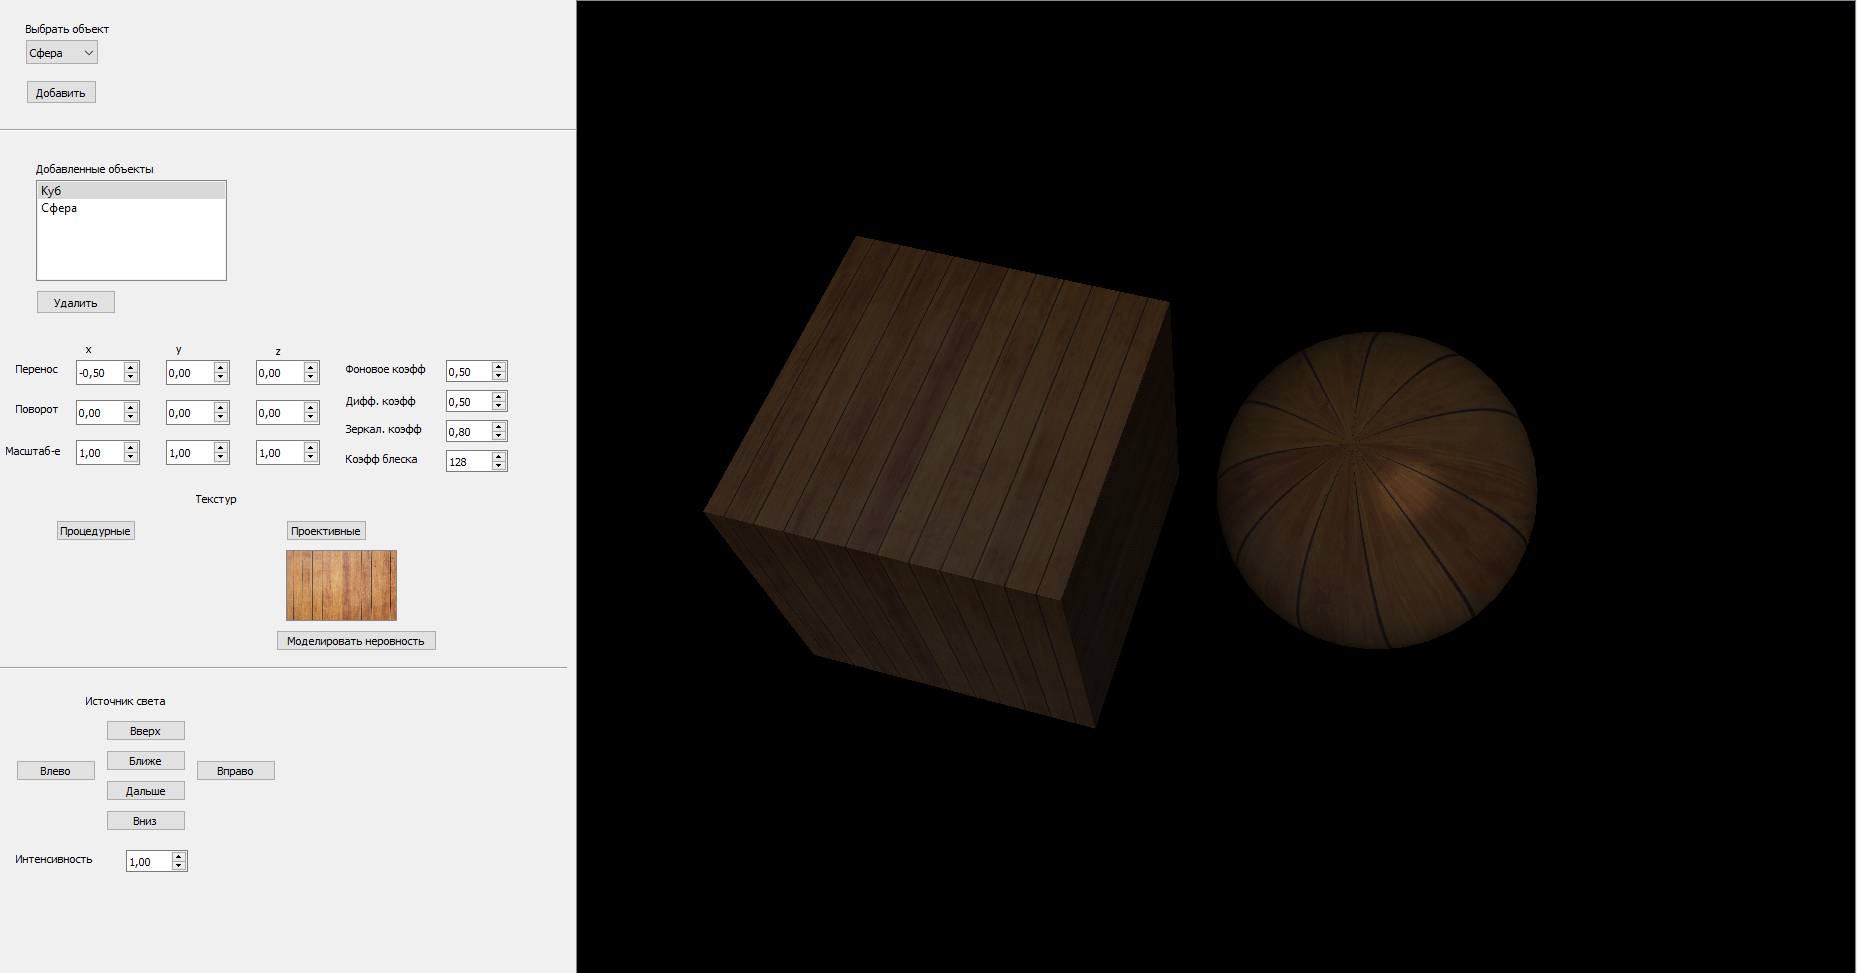
\includegraphics[width=0.95\textwidth]{img/examples/demon2.png}
	\caption{Результат работы программы при наложении текстуры}
	\label{fig:demon2}
\end{figure}

\begin{figure}[h]
	\centering
	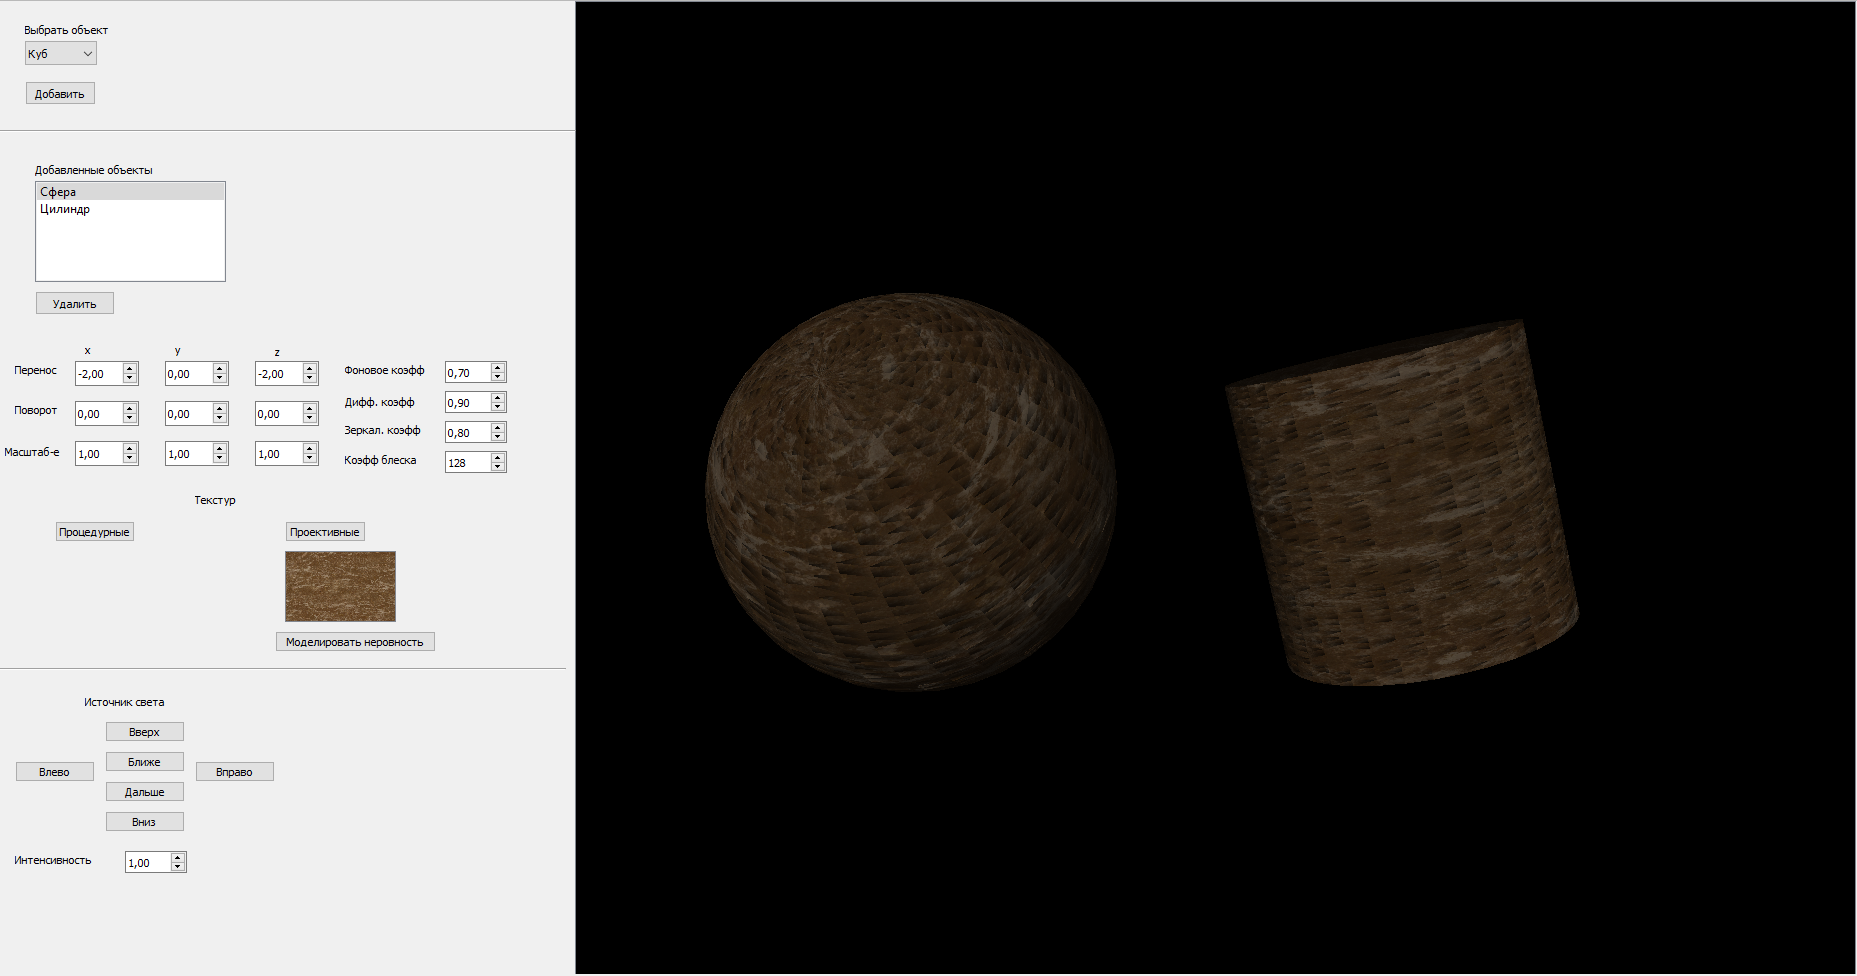
\includegraphics[width=0.95\textwidth]{img/examples/demon3.png}
	\caption{Результат работы программы при моделировании неровностей}
	\label{fig:demon3}
\end{figure}
\clearpage
\subsection*{Вывод}
Было приведено описание структура программы, выбраны средства реализации программного обеспечения, приведены листинги кода, продемонстрирован интерфейс программы и представлены результаты работы программы. 
